\documentclass[a4paper, 12pt]{article}%тип документа

%отступы
\usepackage[left=1.5cm,right=1cm,top=2cm,bottom=3cm,bindingoffset=0cm]{geometry}
\setlength{\parindent}{5ex}

%Русский язык
\usepackage[T2A]{fontenc} %кодировка
\usepackage[utf8]{inputenc} %кодировка исходного кода
\usepackage[english,russian]{babel} %локализация и переносы

%Вставка картинок
\usepackage{graphicx}
\graphicspath{{pictures/}}
\DeclareGraphicsExtensions{.pdf,.png,.jpg,}
\usepackage{wrapfig}

%Графики
\usepackage{pgfplots}
\pgfplotsset{compat=1.9}

%Математика
\usepackage{amsmath, amsfonts, amssymb, amsthm, mathtools}

%Таблицы
\usepackage{longtable} 
\usepackage{float}

%Римские цифры
\newcommand{\RomanNumeralCaps}[1]{\uppercase\expandafter{\romannumeral#1}}

\usepackage{multirow}



\begin{document}
	\begin{titlepage}
		\begin{center}
			\textsc{Федеральное государственное автономное образовательное учреждение высшего образования«Московский физико-технический институт (национальный исследовательский университет)»\\[5mm]
			}
			
			\vfill
			
			\textbf{Отчёт по лабораторной работы 4.3.1\\[3mm]
				ИЗУЧЕНИЕ
				ДИФРАКЦИИ СВЕТА 
				\\[50mm]
			}
			
		\end{center}
		
		\hfill
		\begin{minipage}{.5\textwidth}
			Выполнил студент:\\[2mm]
			Сериков Василий Романович\\[2mm]
			группа: Б03-102\\[5mm]
			
		\end{minipage}
		\vfill
		\begin{center}
			Москва, 2023 г.
		\end{center}
		
	\end{titlepage}
	
	\newpage
	\setcounter{page}{2}
	\textbf{Аннотация}\\
	
	\textbf{Цель работы: }\\
	
	 Исследовать явления дифракции Френеля и Фраунгофера на одной и двух щелях.\\
	 
	 \textbf{В работе используется: }\\
	 
	 Оптическая скамья, ртутная лампа, монохроматор, щели с регулируемой шириной, рамка с вертикальной нитью, двойная щель, микроскоп на поперечных салазках с микрометрическим винтом, зрительная труба.\\
	 
	 \textbf{Теория: }\\
	 
	 \textit{А. Дифракция Френеля}\\
	 
	 
	 \begin{figure}[h]
	 	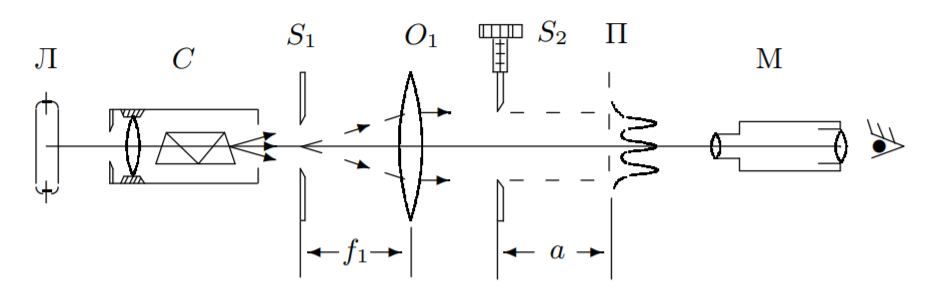
\includegraphics[scale=0.7]{0.png}
	 	\centering
	 	\caption{Схема установки 1.}
	 \end{figure}
	 Схема установки представлена на Рис. 1. Световые лучи освещают щель $S_2$ и испытывают на ней дифракцию. Дифракционная картина рассматривается с помощью микроскопа М, сфокусированного на некоторую плоскость наблюдения П. Щель $S_2$ освещается параллельным пучком монохроматического света с помощью коллиматора, образованного объективом $O_1$ и щелью $S_1$, находящейся в его фокусе. На $S_1$ сфокусированно изображение спектральной линии, выделенной из спектра ртутной лампы Л при помощи монохроматор $C$, в котором используется призма прямого зрения. \\
	 Распределение интенсивности света в плоскости П рассчитаем с помощью зон Френеля. При освещении $S_2$ параллельным пучком лучей (плоская зона) зоны Френеля представляют собой плоскости, параллельные краям щели. Результирующая амплитуда в точке наблюдения определеяется суперпозицией колебаний от тех зон Френеля, которые не перекрыты створками щели. Графическое определение результирующей амплитуды производится с помощью векторной диаграммы -- спирали Корню. Суммарная ширина $m$ зон Френеля $z_m$ определяется соотношение
	 \begin{equation}
	 	z_m = \sqrt{am\lambda},
	 \end{equation}
	 где $a$ -- расстояние от щели до плоскости П. Вид наблюдаемой картины определяется \textit{числом Френеля} $\Phi$:
	 $$
	 \Phi^2 = \dfrac{D}{\sqrt{a\lambda}}
	 $$
	 -- число зон Френеля, которые укладываются в ширине щели $D$. $p = \frac{1}{\Phi^2}$ называется \textit{волновым параметром}. Дифракционной картины нет, когда П совпадает с плоскостью щели. При малом удалении от щели $\Phi \gg 1$ и картина наблюдается в узкой убласти на границе света и тени у краёв экрана. При последующих удалениях две группы дифракционных полос перемещаются независимо и каждая образует картину дифракции Френеля на экране. Распределение интенсивности может быть найдено с помощью спирали Корню. При дальнейшем увеличении $a$ две системы полос сближаются и накладываются друг на друга, распределение интенсивности определяется числом зон Френеля в полуширине щели. Если их $m$, то будет набюдаться $m-1$ тёмная полоса.\\
	 
	 \textit{Б. Дифракция Фраунгофера на щели}\\
	 
	 \begin{wrapfigure}{r}{0.5\textwidth}
	 	\begin{center}
	 		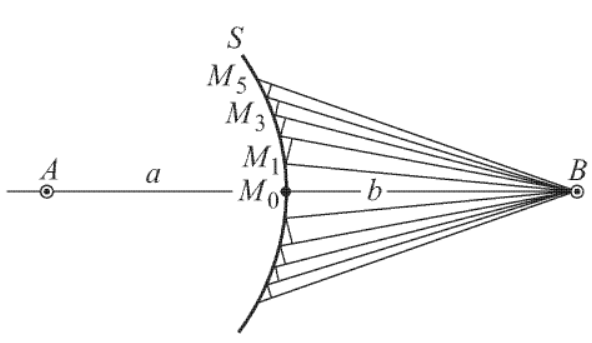
\includegraphics[width = 0.4\textwidth]{2.png}
	 	\end{center}
	 	\caption{Построение зон Френеля}
	 \end{wrapfigure}
	 Для выкладок ниже нам потребуется знать \textit{принцип Гюйгенса-Френеля}. Он формулируется следующим образом:\\
	 \textit{Каждый элемент волнового фронта можно рассматривать как центр  вторичного возмущения, порождающего вторичные сферические волны, а результирующее световое поле  в каждой точке пространства будет определяться интерференцией этих волн.}\\
	 Теперь рассмотрим первое применение этого принципа, получившее название \textit{метод зон Френеля}
	 
	 \begin{wrapfigure}{r}{0.3\textwidth}
	 	\begin{center}
	 		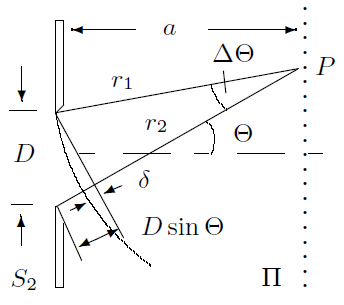
\includegraphics[width = 0.3\textwidth]{1.png}
	 	\end{center}
	 	\caption{К фазовым соотношениям при дифракции Фраунгофера}
	 	\vspace{+30pt}
	 \end{wrapfigure}
	 
	 Для этого рассмотрим действие световой волны действующей из точки $A$ в какой-то точке $B$.
	 В этом случае можно, взяв точку $M_0$ в качестве центра (см. рис. 1), построить ряд концентрических сфер, радиусы которых начинаются с $b$ и увеличиваются каждый раз на половину длины волны $\frac{\lambda}{2}$. При пересечении с плоским фронтом волны $F$ эти сферы дадут концентрические окружности. Таким образом, на фронте волны появятся кольцевые зоны (зоны Френеля) с радиусами $r_1, r_2$ и т. д.
	 
	 Из геометрических соображений посчитав, можно получить, что 
	 \begin{equation}
	 	r_i = i \sqrt{a \lambda}
	 \end{equation}
	 
	 Картина дифракции упрощается, когда ширина щели становится значительно меньше ширины первой зоны Френеля, т.е. если 
	 \begin{equation}
	 	D \ll\sqrt{a \lambda} 
	 \end{equation}	
	 Это условие всегда выполняется при достаточно большом $a$. В этом случае говорят, что \textit{дифракция Фраунгофера}. Дифракционную картину в этом случае называются \textit{дифракцией Фраунгофера}. При выполнении пункта $(2)$ у нас упрощаются фазовые соотношения, что поясняет рис. 2, в итоге с хорошим приближением можно считать, что разность хода между крайними лучами, приходящими от щели в точке наблюдения $P$, с хорошим приближением равна 
	 \begin{equation}
	 	\Delta = r_2 - r_1 \approx D \sin \theta \approx D \cdot \theta
	 \end{equation}
	 Здесь предполагается, что $\theta$ достаточно мал.
	 Дифракцию Фраунгофера можно наблюдать на установке Рис. 1, но для удобства к подобной установке добавляется объектив $O_2$.
	 
	 \begin{figure}[h]
	 	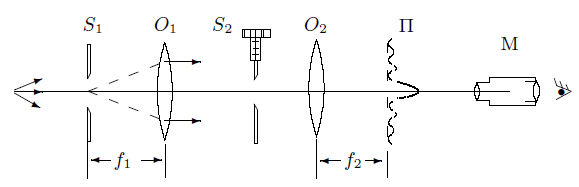
\includegraphics[width = 0.7\textwidth]{3.png}
	 	\centering
	 	\caption{Схема установки 2.}
	 \end{figure}
	 Дифракционная картина здесь наблюдается в фокальной плоскости объектива $O_2$. Каждому значению $\theta$ соответствует в этой плоскости точка, отстоящая от оптической оси на расстоянии 
	 \begin{equation}
	 	X = f_2 \tan \theta \approx f_2 \theta.
	 \end{equation}
	 Объектив не вносит разности хода между интерферирующими лучам, поэтому в его фокальной плоскости наблюдается неискажённая дифракционная картина. При $\theta = 0$ разность хода между лучами нулевая, поэтому в центре поля зрения дифракционный максимум. Первый минимум соответствует $\theta_1$ такому, что в точке наблюдения разность хода пробегаем все значения от 0 до $2\pi$. Аналогично рассуждая, для $m$-й полосы
	 \begin{equation}
	 	\theta_m = \frac{m \lambda}{D}
	 \end{equation}
	 Расстояние $X_m$ тёмной полосы от оптической оси из (5) и (6)
	 \begin{equation}
	 	X_m = f_2m\frac{\lambda}{D}
	 \end{equation} \\
 
 
	 \textit{В. Дифракция Фраунгофера для двух щелей}\\
	 
	 Для наблюдения дифракции Фраунгофера на двух щелях $S_2$ заменим экраном Э с двумя щелями. При этом для оценки влияния ширины входной щели на чёткость вместо $S_1$ поставим щель с микрометрическим винтом.
	 \begin{figure}[h]
	 	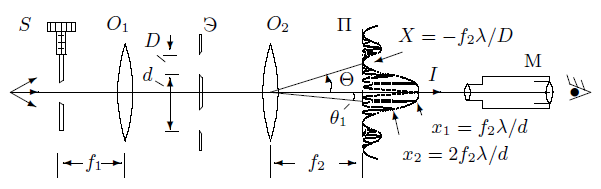
\includegraphics[width = 0.7\textwidth]{4.png}
	 	\centering
	 	\caption{Схема установки 3.}
	 \end{figure}
	 Два дифракционных изображения входной щели, одно из которых образовано лучами, прошедшими через левую, а другое -- через правую щели, накладываются друг на друга.
	 Если входная щель достаточно узка, то дифракционная картина в плоскости П подобна той, что получалась при дифракции на одной щели, однако вся картинка испещерена рядом дополнительных узких полос, наличие которых объясняется суперпозицией световых волн через разные щели. Светлая интерфереционная полоса наблюдается в случаях, когда разность хода равна целому числу длин волн. Таким образом, угловая координата максимума порядка $m$ равна
	 \begin{equation}
	 	\theta_m = \dfrac{m \lambda}{d},
	 \end{equation}
	 где $d$ -- расстояние между щелями. Отсюда расстояние между соседними интерфереционными полосами в плоскости П равно
	 \begin{equation}
	 	\delta x = f_2 \dfrac{\lambda}{d}
	 \end{equation}
	 Число интерференционных полос укладывающихся в области центрального максимума равна отношению ширины главного максимума $\frac{2\lambda f_2}{D}$ к расстоянию между соседними полосами:
	 \begin{equation}
	 	n = \dfrac{2\lambda f_2}{D} \dfrac{1}{\delta f}= \dfrac{2d}{D}.
	 \end{equation}
	 При дифракции света на двух щелях чёткая система интерференционных полос наблюдается только при достаточно узкой ширине входной щели $S$. При увеличении ширины картинка пропадает и появляется вновь, но полосы при этом сильно размыты и видны плохо.\\
	 
	 
	 \textit{Г. Влияние дифракции на разрешающую способность оптического инструмента}\\
	 
	 
	 \begin{figure}[h]
	 	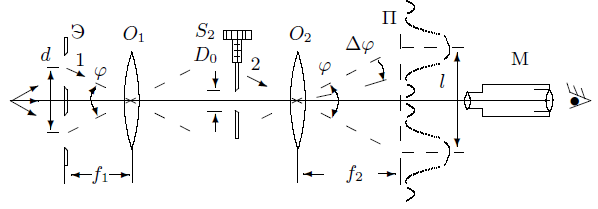
\includegraphics[width = 0.8\textwidth]{5.png}
	 	\centering
	 	\caption{Схема установки 4.}
	 \end{figure}
	 В отсутствие щели $S_2$ линзы $O_1$ и $O_2$ создают на плоскости П изоюражение щели $S_1$ и это изображение рассматриваются микроскопом М. Таким образом, установку можно рассматривать как оптический инструмент, предназначенные для получения изображения предмета. Если перед $O_2$ расположить $S_2$, то изображение объекта будет искажено из-за дифракции. Чем меньше ширина щели, тем сильнее искажение. Качественной характеристикой этого искажения может служить $\varphi_{min}$ --- минимальное угловое расстояние между объектами (источниками), которые всё ещё воспринимаются как раздельные. Поместим вместо $S_1$ экран Э с двумя щелями с расстоянием $d$. Тогда на $S_2$ будут падать два пучка света с углом
	 \begin{equation}
	 	\varphi = \dfrac{d}{f_1}
	 \end{equation}
	 Из геометрии расстояние $l$ между изображениями щелей в плоскости П равно 
	 \begin{equation}
	 	l = \varphi f_2 = d \dfrac{f_2}{f_1}.
	 \end{equation}
	 Ширина $\Delta \varphi$ определяется дифракцией на $S_2$. Условия, при которых изображения различимы разные для разных наблюдателей, поэтому используют \textit{критерий Рэлея} -- \textit{максимум одного дифракционного пятна должен совпадать с минимумом другого}. В наших условиях это значит, что угловая полуширина $\frac{\lambda}{D}$ равна угловому расстоянию $\frac{l}{f_2}$.\\
	 
	 
\textbf{Ход работы: }\\
	 
\textit{А. Дифракция Френеля}\\
	
\begin{enumerate}
	\item Снимем зависимость координаты x
	микроскопа от числа n, ширину $z_m$ m зоны Френеля вычислим по формуле (1). Полученные данные занесем в таблицу 1.
	
	
	\begin{longtable}{|c|c|c|}
		\hline
		m & x, см & $z_m$, мкм  \\ \hline
		1 & 5,35 & 171 \\ \hline
		2 & 3,0 & 181 \\ \hline
		3 & 2,4 & 198 \\ \hline
		4 & 2,0 & 209 \\ \hline
		5 & 1,7 & 215 \\ \hline
		6 & 1,55 & 225 \\ \hline
		7 & 1,3 & 227 \\ \hline
		\caption{Полученные значения положения и ширины m зон Френеля.
		$\sigma_x = 0.05$ см, $\sigma_{z_m} = 10$ мкм}
	\end{longtable}

\item Сравним значение ширины щели измеренной по шкале щели с $2z_0$. 

$$ D = 307 \pm 5 \text{мкм} <=> 2z_0 = 320 \pm 20 \text{мкм}$$ 

\textit{Б. Дифракция Фраунгофера на щели}\\

\item Измерим с помощью винта поперечного перемещения микроскопа координаты $x_m$ нескольких дифракционных минимумов (от -m до +m)

\begin{longtable}{|c|c|}
 	\hline
 	m & $\delta x$, мм\\ \hline
 	1 & 0,10 \\ \hline
 	2 & 0,24 \\ \hline
 	3 & 0,36 \\ \hline
 	4 & 0,48 \\ \hline
 	5 & 0,61 \\ \hline
 	\caption{Полученные значения положения дифракционных минимумов}
\end{longtable}

\item Построим график, откладывая по горизонтали номер минимума m, а по вертикали — его координату $x_m$ (от -m до +m). По углу наклона прямой определим среднее расстояние $\Delta x$ между соседними минимумами; рассчитаем ширину щели D по формуле (7) и сравним с измеренной.

\begin{figure}[H]
 	\center{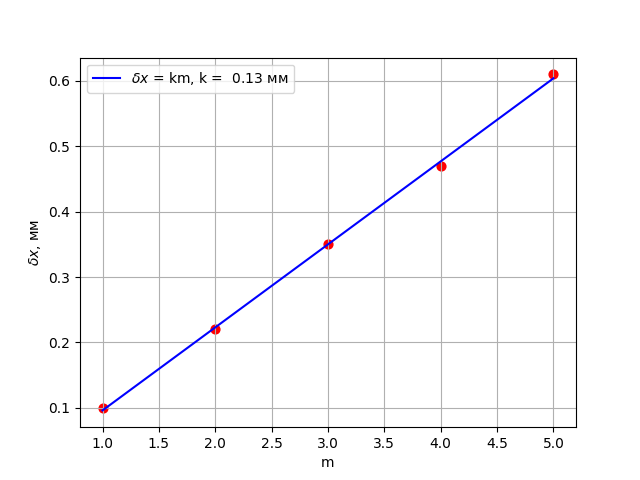
\includegraphics[scale=0.8]{fraungofer1.png}}
 	\caption{График зависимости $\delta x (m)$.}
\end{figure}

$$ \delta x = f_2 \frac{m\lambda}{D} <=> D = f_2 \frac{\lambda}{k} = 370 \pm 20\text{ мкм} $$


$$ D = 309 \pm 5 \text{мкм, расчет по шкале щели} $$\\


\textit{В. Дифракция Фраунгофера для двух щелей}\\

\item Измерим ширину центрального максимума и количество интерференционных максимумов, которые помещаются в него. Определим ширину щели с помощью формулы (9) и сравним с измеренной по микроскопу величиной.

$$ \delta x = f_2 \frac{\lambda}{d} => d = f_2 \frac{\lambda}{\delta x}  = 1,6 \pm 0,1 \text{мм}$$

$$ D = 1,28 \pm 0,02 \text{ мм, измерено по микроскопу} $$

\item Определим ширину щели $S_2$ с помощью формулы $ \frac{b}{f_1} = \frac{\lambda}{D}$ и сравним с величиной измеренной микрометром на щели

$$ b = \frac{\lambda f_1}{D} = 59 \pm 3 \text{ мкм}$$
$$ b = 63 \pm 1 \text{ мкм, измерено с помощью микрометра}$$


\textit{Г. Влияние дифракции на разрешающую способность оптического инструмента}\\

\item Проверим разрешающею способность по критерию Рэлея, для этого сравним ширину измеренную по микрометру щели с расчетом по формуле $\frac{\lambda}{b} < \frac{d}{f_1}$


$$ \frac{b}{\lambda} > \frac{f_1}{d} => b > 59 \pm 3 \text{ мкм}$$\\

\textbf{Обсуждение результатов и выводы: }\\


\begin{longtable}{|c|c|c|c|}
	\hline
 & Френель & Фраунгофер 1 щель & Фраунгофер 2 щели\\ \hline
	Расчет & D = 307$\pm 5$ мкм& D = 370$\pm 20$ мкм &  D$_1$ = 1,6$\pm 1$ мкм\\ 
	& & & b = 59$\pm 3$ мкм \\ \hline
	
	Измерения & D = 320 $\pm 20$ мкм & D = 309$\pm 5$ мкм & D$_1$ = 1,28$\pm 0,02$ мкм\\ 
	& & & b = 63$\pm 1$ мкм\\ \hline

	\caption{Сравнительная таблица. D - ширина щели S$_2$, D$_1$ - расстояние между щелями экрана, b -  ширина щели S$_2$}
\end{longtable}

В данной работе мы исследовали 2 вида дифракции на щели: Френеля и Фраунгофера. По полученным результатам видно, что теория с практикой сходится не во всех опытах. Можно попробовать объяснить это тем, что система может быть плохо отцентрирована или некачественно сняты показания приборов. Также имеет место качество используемых измерительных приборов.


\end{enumerate}
	
\end{document}